\chapter{Related Work}
\label{chap:lit}

This dissertation lies at the intersection of language testing, second language acquisition (SLA), intelligent computer-assisted language learning (ICALL), corpus linguistics and natural language processing (NLP). My work here is much indebted to related research in these areas, and this chapter will summarize some of the most relevant and comparable studies.

I begin in Section~\ref{section:stateOfICALL} with a look at the state of ICALL, its current abilities and limitations, and how it relates generally to this dissertation. In Section~\ref{section:learnerCorpora}, I summarize research involving the collection, annotation or content analysis of task-based learner corpora. A brief overview of the NLP tools and methods used in my work is given in Section~\ref{section:NLP}. Finally, in Section~\ref{section:myPreviousWork}, I present a summary of my own previous related work.

%In this section, I want to discuss related work, including work that involves learner corpora (collecting, annotating for special purposes, etc.).
%
%I also want to discuss work that involves automatically evaluating learner responses to tasks, particularly tasks involving a visual reference.

\section{The state of ICALL and content analysis}
\label{section:stateOfICALL}
My dissertation bears much in common with language testing research, but it began as an experiment in bootstrapping NLP tools and learner data to achieve more meaning-based (and meaningful) ICALL. I do not attempt a full-fledged ICALL system, but I explore mechanisms for implementing content analysis that could be implemented in an interactive setting like a game or an interactive language tutor (ILT). This section examines the current state of ICALL, particularly with regard to visual references and meaning-based interactions.

\section{Learner corpora}
\label{section:learnerCorpora}
Here I will discuss task-based learner corpora research that relates to my work. This includes discussions of task design, data collection, annotation schemes, and automatic processing. I focus in particular on the learner content analysis research conducted by two clusters of researchers: one primarily associated with The Ohio State University and consisting of Detmar Meurers and colleagues, and the other primarily associated with Educational Testing Services (ETS) and consisting of Martin Chodorow, Swapna Somasundaran and Joel Tetrault and colleagues. 

Here are some papers I discussed briefly in my BEA 2018 paper:

\cite{leacock:ea:14}

\cite{kyle2015automatically}

\cite{weigle2013english}

\cite{amaral:meurers:user:07}

\cite{Meurers.Dickinson-17}

\cite{heift:schulze:07}

\cite{somasundaran:ea:15}

\cite{bailey:meurers:08}

\cite{meurers2011evaluating}

\cite{somasundaran:chodorow:14}

\cite{cahill-et-al:14}

\cite{ragheb:dickinson:14a}

\cite{foster2009native}

\cite{cho2013investigating}

\cite{landis1977measurement}

\cite{artstein:massimo:2008}

\cite{tetreault-chodorow:2008:HJCL}

\cite{tetreault:chodorow:08}

\section{Language assessment}
\label{section:languageAssessment}

\section{NLP tools and methods}
\label{section:NLP}

\section{My previous work}
\label{section:myPreviousWork}
Here I will discuss the work I have previously done in this area, including the papers given in the subsections below.

\subsection{2013}
\cite{king:dickinson:13}

\begin{figure}
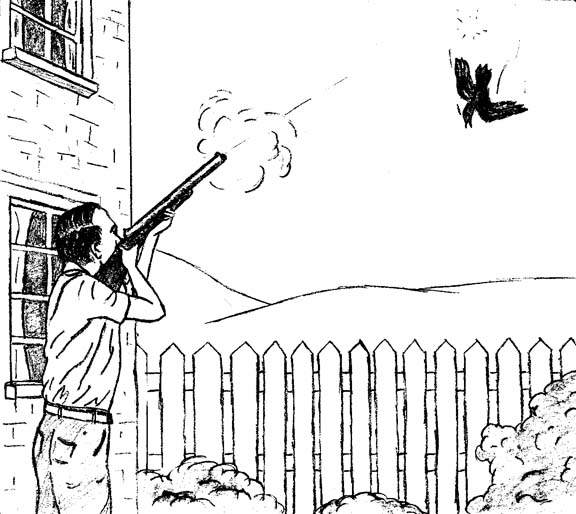
\includegraphics[width=.7\textwidth]{figures/exampleprompt2.jpg}
\caption{This is an example figure from \citet{king:dickinson:13}.}
\label{figure:KandD2013}
\end{figure}

\subsection{2014}
\citet{king:dickinson:14}

\subsection{2016}
\citep{king:dickinson:16}

\subsubsection{Bag-of-dependencies}
Here we could discuss the switch to a bag-of-dependencies approach, the use of tf-idf and the use of vector cosine distance for ranking responses.

\subsubsection{Clustering}
Here we could briefly mention the clustering experiments we did in the 2016 paper. But really, I'd rather not, because I don't intend to repeat them in the dissertation.

\subsection{2018}
\cite{king:dickinson:18}

\begin{figure}

\includegraphics[width=.7\textwidth]{figures/I29.jpg}
\caption{This is an example figure from \citet{king:dickinson:18}.}
\label{figure:KandD2018}
\end{figure}

\section{Image processing}
\label{figure:imageProcessing}
We want to touch on image processing / automatic captioning / use of semantic primatives, etc. -- linguistic annotation of images. NOT a deep discussion, but we need to acknowledge that there are other fields working on the relations between images and text, and give an idea of what some approaches are and how they work, and how they might relate to my work and the work discussed in my lit review.


% This is a figure in landscape orientation
%\begin{sidewaysfigure}
%
\includegraphics[width=\textwidth]{figures/exampleFigure.png}
%\caption{This is another example Figure, rotated to landscape orientation.}
%\label{LandscapeFigure}
%\end{sidewaysfigure}
